\documentclass[
	% -- opções da classe memoir --
	article,			% indica que é um artigo acadêmico
	12pt,				% tamanho da fonte
	oneside,			% para impressão apenas no recto. Oposto a twoside
	a4paper,			% tamanho do papel.
	% -- opções da classe abntex2 --
	%chapter=TITLE,		% títulos de capítulos convertidos em letras maiúsculas
	%section=TITLE,		% títulos de seções convertidos em letras maiúsculas
	%subsection=TITLE,	% títulos de subseções convertidos em letras maiúsculas
	%subsubsection=TITLE % títulos de subsubseções convertidos em letras maiúsculas
	% -- opções do pacote babel --
	english,			% idioma adicional para hifenização
	brazil,				% o último idioma é o principal do documento
	sumario=tradicional
	]{abntex2}


% ---
% PACOTES
% ---

\usepackage{lmodern}			% Usa a fonte Latin Modern
\usepackage[T1]{fontenc}		% Selecao de codigos de fonte.
\usepackage[utf8]{inputenc}		% Codificacao do documento (conversão automática dos acentos)
\usepackage{indentfirst}		% Indenta o primeiro parágrafo de cada seção.
\usepackage{float}
\usepackage{nomencl} 			% Lista de simbolos
\usepackage{color}				% Controle das cores
\usepackage{graphicx}			% Inclusão de gráficos
\usepackage{microtype} 			% para melhorias de justificação
% ---

% ---
% Pacotes de citações
% ---
\usepackage[brazilian,hyperpageref]{backref}	 % Paginas com as citações na bibl
\usepackage[alf]{abntex2cite}	% Citações padrão ABNT
% ---

% ---
%Caminho das imagens
\graphicspath{ {images/} }
% ---

% ---
% Configurações do pacote backref
% Usado sem a opção hyperpageref de backref
\renewcommand{\backrefpagesname}{Citado na(s) página(s):~}
% Texto padrão antes do número das páginas
\renewcommand{\backref}{}
% Define os textos da citação
\renewcommand*{\backrefalt}[4]{
	\ifcase #1 %
		Nenhuma citação no texto.%
	\or
		Citado na página #2.%
	\else
		Citado #1 vezes nas páginas #2.%
	\fi}%
% ---

% ---
% Informações de dados para CAPA e FOLHA DE ROSTO
% ---
\titulo{Criptografia Simétrica D.E.S - Data Encryption Standard}
\autor{
Angelo Rodrigo Ribeiro da Silva\thanks{angelorodriigo.rs@gmail.com} Jaíne da Silva Santos\thanks{jaine.ssilva1@gmail.com}
\\Jonatas Rosa da Silva Bonventi\thanks{jonatasbvt@yahoo.com}
}
\local{Boituva}
\data{2017}

% Configurações de aparência do PDF final

% alterando o aspecto da cor azul
\definecolor{blue}{RGB}{41,5,195}

% informações do PDF
\makeatletter
\hypersetup{
     	%pagebackref=true,
		pdftitle={\@title},
		pdfauthor={\@author},
    	pdfsubject={Análise de vulnerabilidade de redes wifi utilizando técnicas de WarDriving},
	    pdfcreator={LaTeX with abnTeX2},
		pdfkeywords={wardriving}{Wifi}{segurança da informação}{ifsp},
		colorlinks=true,       		% false: boxed links; true: colored links
    	linkcolor=blue,          	% color of internal links
    	citecolor=blue,        		% color of links to bibliography
    	filecolor=magenta,      		% color of file links
		urlcolor=blue,
		bookmarksdepth=4
}
\makeatother


% compila o indice
\makeindex

% Margens segundo abnt
\setlrmarginsandblock{3cm}{3cm}{*}
\setulmarginsandblock{3cm}{3cm}{*}
\checkandfixthelayout

% ---
% Espaçamentos entre linhas e parágrafos
% ---

% O tamanho do parágrafo é dado por:
\setlength{\parindent}{1.3cm}

% Controle do espaçamento entre um parágrafo e outro:
\setlength{\parskip}{0.2cm}  % tente também \onelineskip

% Espaçamento simples
\SingleSpacing

% Início do documento
\begin{document}

% Seleciona o idioma do documento (conforme pacotes do babel)
\selectlanguage{brazil}

% Retira espaço extra obsoleto entre as frases.
\frenchspacing

% ELEMENTOS PRÉ-TEXTUAIS
% página de titulo
\maketitle

% resumo em português
\begin{resumoumacoluna}
 Resumo de uma coluna.

 \vspace{\onelineskip}

 \noindent
 \textbf{Palavras-chave}: Wardriving. Segurança da informação.
\end{resumoumacoluna}

% ELEMENTOS TEXTUAIS
\textual

% Introdução
\section*{Introdução}
\addcontentsline{toc}{section}{Introdução}

Segundo \cite[p. 67]{redes-tanenbaum} "Quase na mesma época em que surgir am os notebooks, muitas pessoas sonhavam com o dia em que entrariam em um escritório e magicamente seu notebook se conectaria à Internet.", e logicamente, veio logo após a necessidade de proteger essas redes através de criptografia e outras técnicas de segurança.

E também, com a melhora de segurança das redes, surgiram pessoas interessadas em quebrar essas redes, seja por interesse financeiro, corporativo ou mesmo pelo triunfo de se atingir um objetivo utilizando técnicas de quebra, prática muito comum nas comunidades de hackers.

\section{Wardriving}

%Jonatas%

\section{Protocolas de segurança em redes sem fio}

\section{Análise de vulnerabilidade e tentativa de quebra de senhas}

Buscando analisar a vulnerabilidade de redes wifi de estabelecimentos, fomos a um shopping em Sorocaba avaliar as redes através de wardriving e depois tentarmos quebrar redes.

\subsection{Objetivos}

O nosso objetivo é verificar se os grandes estabelecimentos se preocupam com segurança de redes, visto que milhares de usuários acessam a rede todos os dias.

\subsection{Ferramentas utilizadas}

\subsubsection{Kismet}

Nós utilizamos o Kismet para realizar wardriving e capturar estátisticas e pacotes das redes wifi e salvar essas informações utilizando gps, para podermos analizar após.

\subsubsection{Wireshark}

Para as redes abertas, decidimos capturar os pacotes enviados e recebidos de toda a rede utilizando wireshark.

\subsubsection{Aircrack}

Para as redes fechadas, com a captura de pacotes, fizemos então handshake, e após, tentativas de quebra utilizando wordlists de 13.2 gb com 1.2 bilhão de senhas.

\subsection{Resultados da análise de redes}

\subsubsection{Captura de pacotes}

Conseguimos capturar através do Kismet 37 redes sem fio válidas (com conexão), das quais 22 eram redes abertas que foram analisadas utilizando sniffing e 15 eram redes privadas.

\begin{figure}[H]
	\centering
	\caption{Gráfico das seguranças de redes sem fio utilizadas.}
	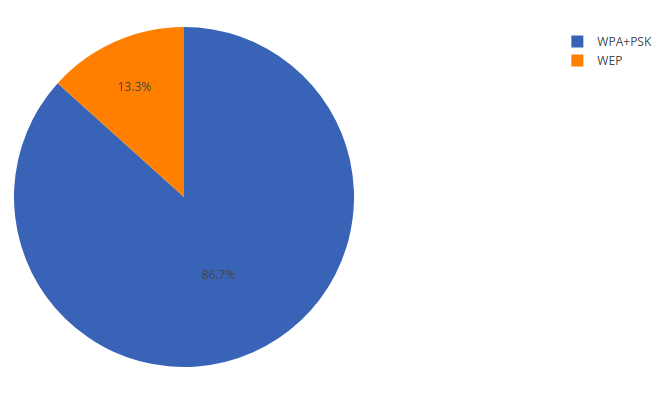
\includegraphics[scale=0.7]{graficopie-seguranca-redes}
\end{figure}

Como podemos ver acima, a maior parte das redes wifi privadas utilizam a criptografia de rede WPA2-PSK, porém ainda temos redes que utizam protocolo WEP, que é muito inseguro e fácil de ser quebrado.

\subsubsection{Cracking de senhas}

Após feita a captura dos pacotes, capturamos os handshakes utilizando o comando aireplay-ng do pacote aircrack.\\

\subsubsubsection{WPA-PSK}

Para redes WPA-PSK, utilizamos um arquivo word-list contendo 1.2 bilhão de senhas mais utilizadas em redes sem fio, utilizando o aircrack-ng.\\

Das redes WPA-PSK analisadas, nenhuma foi quebrada, mesmo após utilizar toda a lista.

\subsubsubsection{WEP}

\subsubsection{Sniffing}

% Finaliza a parte no bookmark do PDF, para que se inicie o bookmark na raiz
\bookmarksetup{startatroot}

% Conclusão
\section*{Considerações finais}
\addcontentsline{toc}{section}{Considerações finais}

Conclusão

% Elementos pós textuais
\postextual

% Titulo e resumo em outro idioma

\titulo{Symmetrical DES Criptography}
\emptythanks
\maketitle

\renewcommand{\resumoname}{Abstract}
\begin{resumoumacoluna}
 \begin{otherlanguage*}{english}
   Abstract

   \vspace{\onelineskip}

   \noindent
   \textbf{Keywords}: Wardriving. Information Security.
 \end{otherlanguage*}
\end{resumoumacoluna}

% Referências bibliográficas
\bibliography{wardriving}

\end{document}
\grid
